\definecolor{shadow}{rgb}{0.54, 0.47, 0.36}

\begin{wrapfigure}{r}{0.5\textwidth}
  \begin{center}
    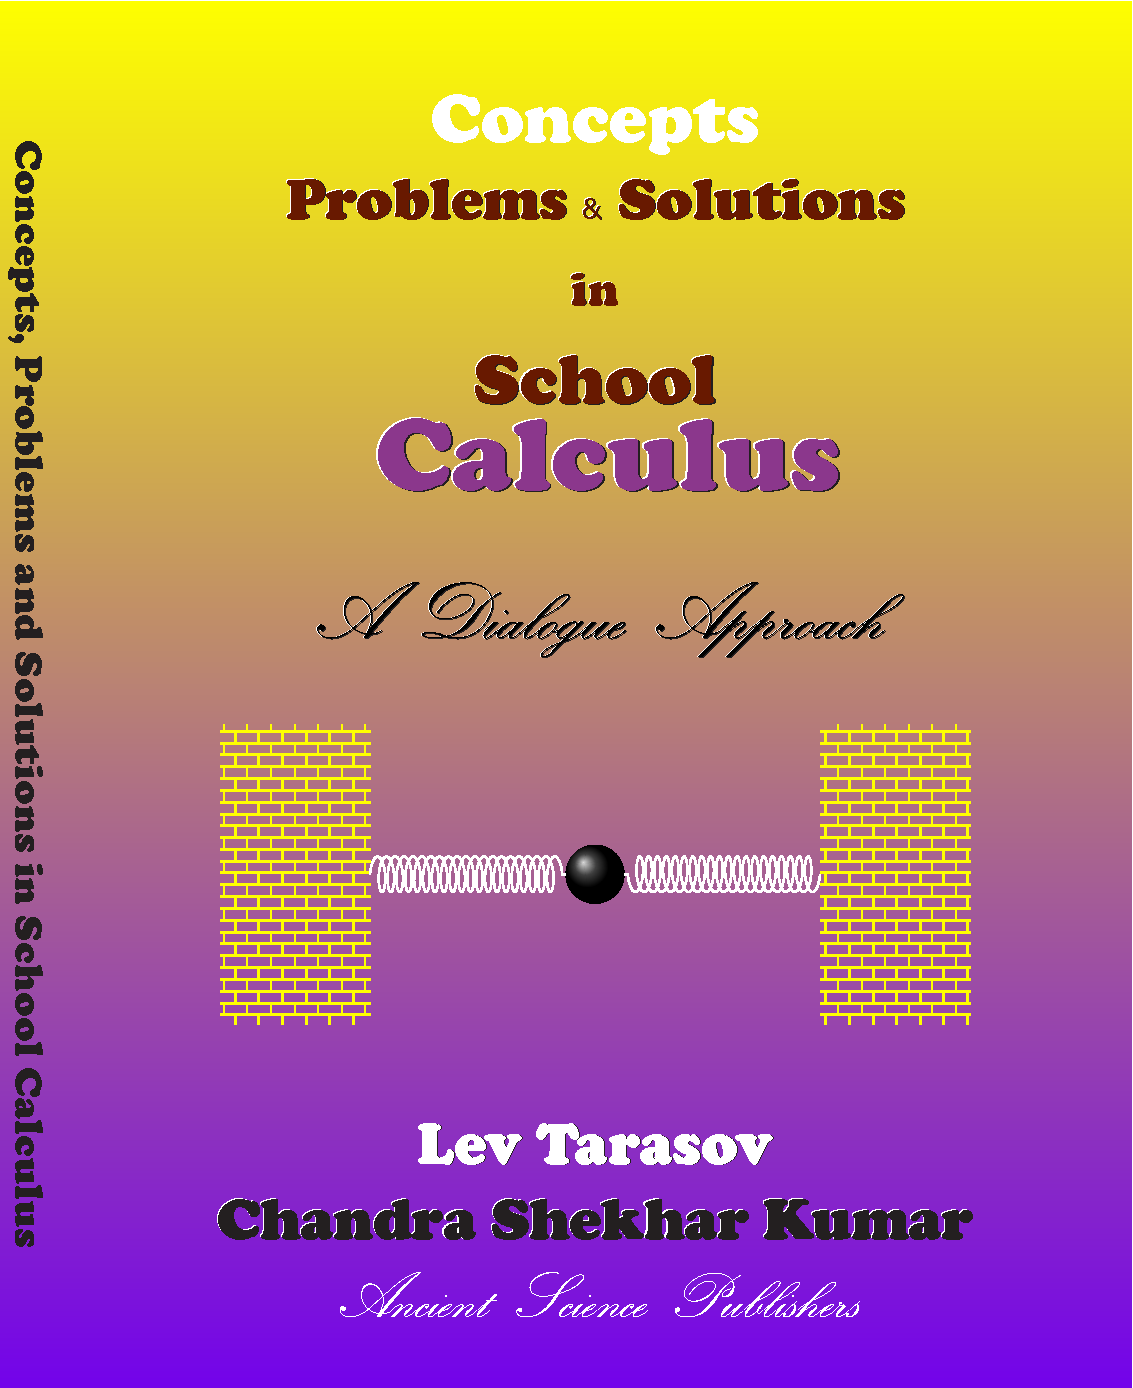
\includegraphics[width=0.5\textwidth]{tarasov-cal/cover}
  \end{center}
  %\caption{Front Cover}
\end{wrapfigure}

\hspace{5mm}\textcolor{shadow}{My first acquaintance with calculus (or mathematical analysis) dates back to nearly a quarter of a century. This happened in the Moscow Engineering Physics Institute during splendid lectures given at that time by Professor D. A. Vasilkov. Even now I remember that feeling of delight and almost happiness. In the discussions with my classmates I rather heatedly insisted on a simile of higher mathematics to literature, which at that time was to me the most admired subject. Sure enough, these comparisons of mine lacked in objectivity. Nevertheless, my arguments were to a certain extent justified. The presence of an inner logic, coherence, dynamics, as well as the use of the most precise words to express a way of thinking, these were the characteristics of the prominent pieces of literature. They were present, in a different form of course, in higher mathematics as well. I remember that all of a sudden elementary mathematics which until that moment had seemed to me very dull and stagnant, turned to be brimming with life and inner motion governed by an impeccable logic.}

\hspace{5mm}\textcolor{shadow}{Years have passed. The elapsed period of time has inevitably erased that highly emotional perception of calculus which has become a working tool for me. However, my memory keeps intact that unusual happy feeling which I experienced at the time of my initiation to this extraordinarily beautiful world of ideas which we call higher mathematics.}

\vspace{2mm}

\begin{center}
\bfseries \underline{\textcolor{Goldenrod}{Confession of The Reader}}
\end{center}

\hspace{5mm}\textcolor{shadow}{Recently our professor of mathematics told us that we begin to study a new subject which he called calculus. He said that this subject is a foundation of higher mathematics and that it is going to be very difficult. We have already studied real numbers, the real line, infinite numerical sequences, and limits of sequences. The professor was indeed right saying that comprehension of the subject would present difficulties. I listen very carefully to his explanations and during the same day study the relevant pages of my textbook. I seem to understand everything, but at the same time have a feeling of a certain dissatisfaction. It is difficult for me to construct a consistent picture out of the pieces obtained in the classroom. It is equally difficult to remember exact wordings and definitions, for example, the definition of the limit of sequence. In other words, I fail to grasp something very important.}

\hspace{5mm}\textcolor{shadow}{Perhaps, all things will become clearer in the future, but so far calculus has not become an open book for me. Moreover, I do not see any substantial difference between calculus and algebra. It seems that everything has become rather difficult to perceive and even more difficult to keep in my memory.}

\vspace{2mm}


\begin{center}
\bfseries \underline{\textcolor{Goldenrod}{Comments of The Author}}
\end{center}

\hspace{5mm}\textcolor{shadow}{These two confessions provide an opportunity to get acquainted with the two interlocutors in this book. In fact, the whole book is presented as a relatively free-flowing dialogue between the \hlt{author} and the \hlt{reader}. From one discussion to another the \hlt{author} will lead the inquisitive and receptive \hlt{reader} to different notions, ideas, and theorems of calculus, emphasizing especially complicated or delicate aspects, stressing the inner logic of proofs, and attracting the reader's attention to special points. I hope that this form of presentation will help a reader of the book in learning new definitions such as those of \hlt{derivative, anti-derivative, definite integral, differential equation}, etc. I also expect that it will lead the reader to better understanding of such concepts as numerical sequence, limit of sequence, and function. Briefly, these discussions are intended to assist pupils entering a novel world of calculus. And if in the long run the reader of the book gets a feeling of the intrinsic beauty and integrity of higher mathematics or even is appealed to it, the author will consider his mission as successfully completed.}

\hspace{5mm}\textcolor{shadow}{Working on this book, the author consulted the existing manuals and textbooks such as \hlt{Algebra and Elements of Analysis} edited by A. N. Kolmogorov, as well as the specialized textbook by N. Ya. Vilenkin and S. I. Shvartsburd \hlt{Calculus}. Appreciable help was given to the author in the form of comments and recommendations by N. Ya. Vilenkin, B. M. Ivlev, A. M. Kisin, S. N. Krachkovsky, and N. Ch. Krutitskaya, who read the first version of the manuscript. I wish to express gratitude for their advice and interest in my  work. I am especially grateful to A. N. Tarasova for her help in preparing the manuscript.}

\vspace{0.2in}

 \hfill \emph{\color{Sepia} \textbf{Lev Tarasova}}

\vspace{0.2in}

\thispagestyle{empty}

\hspace{5mm}\textcolor{shadow}{In this edition, the entire manuscript was typeset using the \LaTeXe{} document processing system originally developed by \emph{Leslie Lamport}, based on \TeX{} typesetting system created by \emph{Donald Knuth}. The typesetting software used the \hologo{XeLaTeX} distribution.}

\hspace{5mm}\textcolor{shadow}{Employing the extremely lively form of dialogue, almost all the subjects in the syllabus are discussed comprehensively, especially questions usually considered difficult to understand. The book presents a detailed analysis of common mistakes made by students embarking on learning and applying concepts in calculus. Students will find this to be an exceptionally clear and interesting textbook which treats of  complicated problems from various viewpoints and contains a great many excellent illustrations promoting a deeper  understanding of the ideas and concepts involved.}

\hspace{5mm}\textcolor{shadow}{I am grateful for this opportunity to put the materials into a consistent format, and to correct errors in the original publication that have come to my attention. The process of compiling this book has given me an incentive to improve the text, dialogue, concepts, problems, solutions, layout, to double check almost all of the mathematical rendering, to correct all known errors, to improve the original illustrations by redrawing them with Till Tantau's marvellous \textup{Ti\textit{k}Z}. Thus the book now appears in a form that we hope will remain useful for at least another generation.}


\thispagestyle{empty}

\vspace{3mm}

\noindent {\calligra Ancient Science Publishers}  \hfill \emph{\color{Sepia} \textbf{Chandra Shekhar Kumar}}


\begin{center}\bfseries \large
\textcolor{Gold}{Author}  \\
\textcolor{BurntOrange}{Reader} 
\end{center}

\section{Table of Contents}
%\begin{comment}
\begin{enumerate}[nosep]
\item Infinite Numerical Sequence
\item Limit Of Sequence
\item Convergent Sequence 
\item Function
\item More On Function
\item Limit of Function
\item More on The Limit of Function
\item Velocity
\item Derivative
\item Differentiation
\item AntiDerivative
\item Integral
\item Differential Equations
\item More On Differential Equations
\item Problems
\end{enumerate}
%\end{comment}

\hrulefill

\newtheorem{probl}{\textcolor{Gold}{\textbf{\textsc{Author}}}}[chapter]

\renewenvironment{p}    % this is the environment name for the input
  {\renewcommand{\qedsymbol}{$\lozenge$}%
   \pushQED{\qed}\begin{probl}}
  {\popQED\end{probl}}
  
\renewenvironment{s}
  {\renewcommand{\qedsymbol}{\tiny$\blacksquare$}
  \vspace{-\baselineskip}
  \begin{proof}[\emph{\textbf{\scshape \textcolor{BurntOrange}{Reader}}}]\color{zinnwalditebrown}}
  {\end{proof}} 

\underline{\textbf{\textcolor{BurntOrange}{Excerpt from the Chapter} \textcolor{Sepia}{7:}}}

\section{More on The Limit of Function}


\begin{s} 
Comparing the definition of the limit of a function at a point with the definition of the limit of a numerical sequence, I come to the conclusion that these two limits are of different nature.
\end{s}


\begin{p}
And I understand why. In fact, I did emphasize the difference myself in the previous dialogue, pointing out, as you probably remember, that a sequence is a function defined on a set of integers, while the functions we are discussing at the moment are defined over intervals. I doubt, however, that you are justified in speaking about the difference in the nature of the limit of function and that of sequence. In the final analysis (and this is essential) \hlt{the limit of a function at a point may be defined on the basis of the limit of a numerical sequence}.
\end{p}

\begin{s}
This is very interesting.
\end{s}

\begin{p}
Let us forget, for the time being, about the definition of the limit of function given in the previous dialogue. Consider a new definition. 

We shall consider, as before, a function, \hlm{$f (x)$} defined over an interval, and a point \hlm{$x = a$} either taken within the interval or coinciding with its end.

The definition of the limit of function may be formulated as follows.

\begin{defn}
A number \hlm{$b$} is said to be the limit of a function \hlm{$f(x)$} at a point \hlm{$x = a$} if for any numerical sequence (\hlm{$x_n$}) satisfying the conditions :
\begin{enumerate}[nosep, label=(\arabic*)]
  \item all \hlm{$x_n$} belong to the domain of the function,
  \item \hlm{$x_n \neq a$} for any \hlm{$n$},
  \item the sequence (\hlm{$x_n$}) is convergent and its limit is \hlm{$a$}; the sequence of the corresponding values of the function (the sequence \hlm{$f(x_n)$}) is convergent and its limit is \hlm{$b$}.
  \end{enumerate}
\par\vspace{-1.4\baselineskip}
\qedhere
\end{defn}

So we should \hlt{construct} a sequence convergent to \hlm{$a$} :
\hlm{\begin{gather*}
x_1, \quad x_2, \quad x_3, \quad \ldots, \quad x_n, \quad \ldots
\end{gather*}}
(we assume that all \hlm{$x_n$} belong to the domain of the function and \hlm{$x_n \neq a$} for any \hlm{$n$}). This sequence automatically generates a sequence of the values of the function :
\hlm{\begin{gather*}
f(x_1), \quad f(x_2), \quad f(x_3), \quad\ldots, \quad f(x_n), \quad\ldots
\end{gather*}}

Assume that this sequence is convergent and its limit is \hlm{$b$}. Then let us \hlt{construct} a new sequence convergent to \hlm{$a$}
\hlm{\begin{gather*}
x'_1, \quad x'_2, \quad x'_3, \quad\ldots, \quad x'_n, \quad\ldots
\end{gather*}}
(all \hlm{$x'_n$} belong to the domain of the function; \hlm{$x'_n \neq a$}). It is important that, as in the previous case, the corresponding sequence of the values of the function
\hlm{\begin{gather*}
f(x'_1), \quad f(x'_2), \quad f(x'_3), \quad\ldots, \quad f(x'_n), \quad\ldots
\end{gather*}}
be convergent to \hlm{$b$}. Then we \hlt{construct} a third sequence convergent to \hlm{$a$}
\hlm{\begin{gather*}
x''_1, \quad x''_2, \quad x''_3, \quad\ldots, \quad x''_n, \quad\ldots
\end{gather*}}
and so on. If we find that for \hlt{any} sequence (\hlm{$x_n$}) convergent to \hlm{$a$} (all \hlm{$x_n$} belong to the domain of the function; \hlm{$x_n \neq a$} for any \hlm{$n$}) there is the corresponding sequence of the values of the function convergent to \hlm{$b$}, then \hlm{$b$} is said to be the limit of the function \hlm{$f(x)$} at \hlm{$x = a$}.
\end{p}

\begin{s}
The definition of the limit of function is quite understandable in itself. But how does it relate to our former definition of the limit of function ?
\end{s}

\begin{p}
The two are \hlt{equivalent}. 
\end{p}

\begin{s}
But in form they are quite different.
\end{s}

\begin{p}
We can prove their equivalence. To begin with, let the definition using a \hlm{$\delta$}-neighbourhood of point \hlm{$a$} be called \hlt{definition 1}, and the definition using numerical sequences, \hlt{definition 2}. \index{$\delta$-neighbourhood}

Now, what two theorems must be proved to demonstrate the equivalence of definitions \hlt{1} and \hlt{2}? Can you formulate these theorems?
\end{p}

\begin{s}
We have to prove two theorems, one direct and the other converse. We want to prove that definition \hlt{2} follows from definition \hlt{1} and vice versa (i.e. definition \hlt{1} follows from definition \hlt{2}).
\end{s}


\begin{p}
Correct. First, I shall prove the following theorem.
\begin{thm}
If a number \hlm{$b$} is the limit of a function \hlm{$f (x)$} at a point \hlm{$a$}, in terms of definition \hlt{1}, it is the limit of the function \hlm{$f (x)$} at \hlm{$a$} in terms of definition \hlt{2} as well.
\end{thm}

Since \hlm{$b$} is the limit of the function \hlm{$f (x)$} at point \hlm{$a$} in terms of definition \hlt{1} (this is given), consequently, for any \hlm{$\varepsilon > 0$} there is \hlm{$\delta > 0$} such that \hlm{$| f(x) - b | < \varepsilon$} for all \hlm{$x \neq a$} from a \hlm{$\delta$}-neighbourhood of point \hlm{$a$}. Then we \hlt{construct} an arbitrary sequence (\hlm{$x_{n}$}), requiring that it be convergent to point \hlm{$a$} (any \hlm{$x_{n}$} belong to the domain of the function and \hlm{$x_{n} \neq a$} for any \hlm{$n$}). As a result we obtain a sequence of the corresponding values of the function (the sequence \hlm{$[f (x_{n} ) ]$}). We want	to prove that the sequence \hlm{$[f (x_{n})]$} is convergent to \hlm{$b$}.

First, I select an arbitrary \hlm{$\varepsilon > 0$}. I should find a number \hlm{$N$} such that \hlm{$|f(x_{n}) - b| < \varepsilon$} for all \hlm{$n > N$}.

I cannot immediately find such \hlm{$N$} for an arbitrary \hlm{$\varepsilon$}. However, I can indicate for an arbitrary \hlm{$\varepsilon$} such \hlm{$\delta$} that \hlm{$| f(x) - b | < \varepsilon$} if \hlm{$|x- a| < \delta$}. Then I take this \hlm{$\delta$} and find a sequence \hlm{$(x_{n})$} convergent to \hlm{$a$}. Evidently, since \hlm{$(x_{n})$} is convergent to \hlm{$a$}, \hlm{$\delta$} (as any other positive real number) can be placed in correspondence with a number \hlm{$N$} such that \hlm{$|x_{n} - a| < \delta$} for all \hlm{$n > N$}. And, consequently, we also have that \hlm{$|f(x_{n}) - b| < \varepsilon$} for all \hlm{$n > N$}. Hence we find that the thus found number \hlm{$N$} is actually the desired number. It proves	the	convergence of the sequence \hlm{$[f (x_{n})]$} to \hlm{$b$}. Since the sequence \hlm{$(x_{n})$},	which is convergent to \hlm{$a$} was chosen (\hlt{constructed}) arbitrarily, we conclude that the theorem's proof is completed.

If the line of reasoning is clear to you, try briefly to recapitulate the logical structure of the proof.
\end{p}

\begin{figure}[H]

\centering

\begin{tikzpicture}[,>=stealth,thick,node distance=10mm, text height=1.5ex, text depth=0.25ex,
    exp/.style={
        rounded rectangle,
        minimum size=6mm,
        ultra thick,
        draw=Black, % border
        top color=Snow,
        bottom color=Grey,
        drop shadow,
        text=Black
    },
    num/.style={
        rounded rectangle,
        minimum size=6mm,
        ultra thick,
        draw=Black, % border
        top color=Snow,
        bottom color=DarkGrey,
        drop shadow,
        text=Black
    }
    ]    
    \node (a) [exp] {$\varepsilon > 0$};
    \node (b) [exp,right=of a] {$\delta > 0$}; 
    
    \path (a) edge[-{latex},line width=2.5pt,in=90,out=-90,color=Grey] (b);
    
    \node (c) [num,below=of a,yshift=-4cm] {$\delta > 0$};
    \node (d) [num,right=of c,xshift=4mm] {$N$};
    
    \path (c) edge[-{latex},line width=2.5pt,in=90,out=-90,color=Grey] (d);
    
    \node (e) [exp,right=of b,draw=none] {};
    \node (f) [exp,above right=of e] {$|x - a| < \delta$};
    \node (g) [exp,below right=of e] {$|f(x) - b| < \varepsilon$};
    
    \path (f) edge[-{latex},line width=2.5pt,in=90,out=-90,color=Grey] (g);
    
    \node (h) [num,right=of d,xshift=3mm,draw=none] {};
    \node (i) [num,above right=of h] {$n > N$};
    \node (j) [num,below right=of h] {$|x_n - a| < \delta$};
    
    \path (i) edge[-{latex},line width=2.5pt,in=90,out=-90,color=Grey] (j);
    
    \node (k) [num,right=of j] {$|f(x_n) - b| < \epsilon$};
    
    \path (j) edge[-{latex},line width=2.5pt,in=90,out=-90,color=Grey] (k);
    
    \path (5.95,0) edge[-{latex},line width=2.5pt,in=90,out=0,color=Grey] (7.6,-7.1);
        
    %\node[drop shadow, ball color=Snow, draw] at (-2,0) {$\varepsilon > 0$};
    %\node at (0,0) {$\delta > 0$};
    
    %\shade[top color=Snow, bottom color=Orange] (0,0) rectangle +(2,1);
\end{tikzpicture}

%\smartdiagramset{back arrow disabled=true}
%\smartdiagram[flow diagram:horizontal]{$\varepsilon > 0$, $\delta > 0$}
%\smartdiagram[flow diagram:horizontal]{$\delta > 0$, $N$}
%\smartdiagram[flow diagram]{$|x - a| < \delta$, $|f(x) - b| < \varepsilon$}
\begin{comment}
\begin{tikzpicture}
    \matrix[matrix of nodes, column sep=5mm, row sep=5mm]
    {
                                           &                         & $|x - a| < \delta$                 &                                                     & \\
        $\varepsilon > 0$ & $\delta > 0$ &                                                 &                                                     & \\
                                           &                          & $|f(x) - b| < \varepsilon$ &                                                     & \\
                                           &                          & $n> N$                                  &                                                     & \\
        $\delta > 0$           & $N$                  &                                                &                                                     & \\
                                           &                          & $|x_n - a| < \delta$            & $|f(x_n) - b| < \varepsilon$ & \\
    };
\end{tikzpicture}
\end{comment}
\caption{Diagrammatic Proof of Equality of Limit of a function via two definitions.}
\label{fig-30}
\end{figure}
\index{Limit of Function!Definitions!Proof of Equality}
%\begin{figure}[!ht]%[13]{r}{0.5\textwidth}
%\centering
%\includegraphics[width=\textwidth]{figures/fig-30.pdf}
%\caption{Schematic diagram of the proof that two definitions of the limit of a function are equal.}
%\label{fig-30}
%\end{figure}


\begin{s}
I shall try to present the structure of the proof as a diagram (\ref{fig-30}).
\end{s}

\begin{p}
Your diagram is correct. Will you expand on it. 
\end{p}

\begin{s}
The \hlt{first step} of the proof: we find for an arbitrary \hlm{$\varepsilon > 0$} a number \hlm{$\delta > 0$} such that \hlm{$| f(x) - b | < \varepsilon$} if \hlm{$|x - a| < \delta$}. 

The \hlt{second step} of the proof: we take \hlm{$\delta$} selected at the first step; choose a sequence \hlm{$(x_{n})$} convergent to \hlm{$a$}, and find a number \hlm{$N$} such that \hlm{$|x - a| < \delta$} for all \hlm{$n > N$}. Having in mind the arguments used at the first step, we conclude that \hlm{$| f(x) - b| < \varepsilon$}. 

We have thus found for an arbitrary \hlm{$\varepsilon > 0$} a number \hlm{$N$} such that \hlm{$| f(x_{n}) - b | < \varepsilon$} for all \hlm{$n > N$}. This completes the proof.
\end{s}

\begin{p}
Correct. In conclusion I want to emphasize several essential points on which the proof hinges. We know that \hlm{$| f(x) - b | < \varepsilon$} for any \hlm{$x$} from the \hlm{$\delta$}-neighbourood of \hlm{$a$}. Since a sequence \hlm{$(x_{n})$} is convergent to \hlm{$a$}, all \hlm{$x_{n}$} (the whole infinite \hlt{tail} of the sequence \hlm{$(x_{n})$} starting from a certain number \hlm{$N +1$}) are contained inside the \hlm{$\delta$}-neighbourhood of point \hlm{$a$}. It then follows that all \hlm{$f (x_{n} )$} (the whole infinite \hlt{tail} of the sequence \hlm{$[f (x_{n})]$} starting from the same number \hlm{$N + 1$}) are contained inside the interval \hlm{$] b - \varepsilon, \; b + \varepsilon[$}, This proves that the sequence \hlm{$[f (x_{n})]$} converges to \hlm{$b$}.
\end{p}

\begin{s}
I understand.
\end{s}


\begin{p}
Now I am going to prove the following converse theorem.
\begin{thm}
If a number \hlm{$b$} is the limit of a function \hlm{$f (x)$} at a point \hlm{$a$} in terms of definition \hlt{2}, it is also the limit of the function \hlm{$f (x)$} at \hlm{$a$} in terms of definition \hlt{1}.
\end{thm}
In this case I shall use the proof by contradiction. Assume the contrary to what is to be proved, namely, assume that \hlm{$b$}, the limit of \hlm{$f (x)$} in terms of definition \hlt{2}, is not, however, the limit of \hlm{$f (x)$} in terms of definition \hlt{1}. Can you formulate the last proposition (more exactly, the assumption)?
\end{p}

\begin{s}
As far as I remember, a similar formulation has already been discussed in the previous dialogue. If \hlm{$b$} is not the limit of the function \hlm{$f (x)$} at point \hlm{$a$} (in terms of definition \hlt{1}), it means that there is \hlm{$\varepsilon' > 0$} such that it is impossible to find a necessary \hlm{$\delta > 0$}. Namely, no matter what \hlm{$\delta$} we select, each time the function \hlm{$f (x)$} assumes a value outside of \hlm{$]b - \varepsilon', \, b + \varepsilon'[$} for at least one point \hlm{$x$} from the \hlm{$\delta$}-neighbourhood of point \hlm{$a$}, i.e. the inequality \hlm{$| f(x) - b | < \varepsilon'$} is violated.
\end{s}

\begin{p}
Correct. Assume that we have selected precisely this \hlm{$\varepsilon' > 0$}. Next take an arbitrary \hlm{$\delta> 0$}, for instance, \hlm{$\delta_{1} = 1$}. As you have said, in any \hlm{$\delta$}-neighbourhood of point \hlm{$a$} and, hence, in the \hlm{$\delta$}-neighbourhood of this point there is at least one point \hlm{$x$} (denoted by \hlm{$x_{1}$}) such that \hlm{$|f(x_{1} - b|  \geqslant \varepsilon'$}.
\end{p}

\begin{s}
What happens if the \hlm{$\delta$}-neighbourhood contains many such points \hlm{$x$}?
\end{s} 


\begin{p}
It makes no difference. The important fact is that there is \hlt{at least one such point}. If there are several such points, take anyone of them and denote it by \hlm{$x_{1}$}.

Now we take a new \hlm{$\delta$}, for instance, \hlm{$\delta_{2} = \dfrac{1}{2}$}. According to our assumption, the \hlm{$\delta_{2}$}-neighbourhood of point \hlm{$a$} will contain at least one point \hlm{$x$} (denoted by \hlm{$x_{2}$}) such that \hlm{$|f(x_{2} - b | \geqslant \varepsilon'$}.

Further we take \hlm{$\delta_{3} = \dfrac{1}{3}$}. The \hlm{$\delta_{3}$}-neighbourhood of point \hlm{$a$} will also contain at least one point \hlm{$x$} (point \hlm{$x_{3}$}) such that \hlm{$|f(x_{3} - b|  \geqslant \varepsilon'$}.

We can continue this process for a sequence of the \hlm{$\delta$}-neighbourhoods of point \hlm{$a$} \hlm{\begin{equation*}%
\delta_{1} = 1, \,\, \delta_{2} = \dfrac{1}{2}, \,\, \delta_{3} = \dfrac{1}{3}, \,\, \ldots \delta_{n} = \dfrac{1}{n}, \,\, \ldots
\end{equation*}}
Note that the \hlm{$\delta$}-neighbourhoods are selected in such a way that the sequence (\hlm{$\delta_{n}$}) converges to zero (is infinitesimal).

If each time we select from each \hlm{$\delta$}-neighbourhood one point \hlm{$x$} in which \hlm{$f (x)$} assumes a value outside of the interval \hlm{$]b - \varepsilon', \, b + \varepsilon'[$}, we obtain a sequence composed of points
\hlm{\begin{equation*}%
x_{1}, \, x_{3}, \, x_{3}, \, \ldots \, x_{n}, \ldots
\end{equation*}}
Since the sequence (\hlm{$\delta_{n}$}) converges to zero, the sequence \hlm{$(x_{n})$} inevitably converges to \hlm{$a$}. A sequence composed of the corresponding values of the function (the sequence \hlm{$[f (x_{n})]$} is not convergent to \hlm{$b$} because for all \hlm{$n$} we have \hlm{$|f(x_{n} - b | \geqslant \varepsilon'$}. It means that we obtained a sequence \hlm{$(x_{n})$} convergent to \hlm{$a$} for which the sequence \hlm{$[f (x_{n})]$} is divergent.

This contradicts the condition of the theorem which states that \hlm{$b$} is the limit of the function at \hlm{$a$} in terms of definition \hlt{2}. It means that for any sequence \hlm{$(x_{n})$} convergent to \hlm{$a$} the corresponding sequence \hlm{$[f (x_{n})$} must be convergent to \hlm{$b$}. And the sequence \hlm{$(x_{n})$} that we have found contradicts this condition.

Hence, the assumption that \hlm{$b$}, being the limit of the function in terms of definition \hlt{2}, is not at the same time the limit of the function in terms of definition \hlt{1}, is invalidated. This completes the proof of the theorem.
\end{p}

\begin{s}
I must admit of being wrong when I spoke about different natures, of the limit of numerical sequence and the limit of function at a point.
\end{s}

\begin{p}
These limits differ but \hlt{their nature is the same}. The concept of the \hlt{limit of function at a point} is based, as we have seen, on the concept of the \hlt{limit of numerical sequence}.

That is why basic theorems about the limits of functions are analogous to those about the limits of sequences.
\end{p}

\begin{s}
We have already noted one of such theorems: the \hlt{theorem on the uniqueness of the limit of function at a point}.
\end{s}


\begin{p}
This theorem is analogous to that about the uniqueness of the limit of numerical sequence.

I shall also give (without proof) the \hlt{theorems on the limit of the sum; the product, and the ratio of functions}. \index{Limit of Function!Sum}\index{Limit of Function!Product}\index{Limit of Function!Ratio}

\begin{thm}
If functions \hlm{$f(x)$} and \hlm{$g(x)$} have limits at a point \hlm{$a$}, then functions
\hlm{\begin{equation*}%
\left[f (x) + g (x) \right], \,\, \left[f (x) g (x) \right], \,\, \left( \frac{f(x)}{g(x)} \right)
\end{equation*}}
also have limits at this point. These limits equal the sum, product, and ratio, respectively, of the limits of the constituent functions (in the last case it is necessary that the limit of the function \hlm{$g (x)$} at \hlm{$a$} be different from zero).
\end{thm}
Thus,
\hlm{
\begin{align*}
\lim\limits_{x \to a} [f (x) +g (x)] & = \lim\limits_{x \to a} f (x) + \lim\limits_{x \to a} g (x)\\[5pt]
\lim\limits_{x \to a} [f(x) \, g(x)]& = \lim\limits_{x \to a} f(x) \, \lim\limits_{x \to a} g(x)\\[5pt]
\lim\limits_{x \to a} \left( \frac{f(x)}{g(x)} \right) & = \frac{\lim\limits_{x \to a} f(x)}{\lim\limits_{x \to a} g(x)} \\[5pt]
& \text{under an additional condition} \,\, \lim\limits_{x \to a} g(x) \neq 0
\end{align*}}
\end{p}

\begin{s}
We have already discussed the similar theorems for numerical sequences.
\end{s}


\begin{p}
Next I wish to make two remarks, using selected examples specially for the purpose.

\textbf{\hlt{Note 1.}} It is illustrated by the following example. Obviously
\hlm{\begin{equation*}%
 \lim\limits_{x \to a} \sqrt{1 - x^{2}} = 0 \,\, \text{and} \,\,  \lim\limits_{x \to a} \sqrt{x - 1} = 0.
  \end{equation*}}
Does it mean that \hlm{$\lim\limits_{x \to a} ( \sqrt{1 - x^{2}} + \sqrt{x - 1}) = 0$}? 
\end{p}


\begin{s}
The limit of the function \hlm{$f(x) = \sqrt{1 - x^{2}}$} at \hlm{$x = 1$} exists and is equal to zero. The limit of the function \hlm{$g(x) = \sqrt{x - 1}$} at \hlm{$x = 1$} also exists and is also equal to zero. According to the theorem on the limit of the sum, the limit of \hlm{$f (x) + g(x) = \sqrt{1 - x^{2}} + \sqrt{x - 1}$} must exist and be equal to the sum of the two preceding limits, i.e. to zero.
\end{s}

\begin{p}
Nevertheless, \hlm{$f (x) + g(x) = \sqrt{1 - x^{2}} + \sqrt{x - 1}$} no limit at \hlm{$x = 1$} for a simple reason that the expression \hlm{$\sqrt{1 - x^{2}} + \sqrt{x - 1}$} has meaning only at a single point (point \hlm{$x = 1$}). Applying the theorem on the limit of the sum, you have not taken into account the domains of the functions \hlm{$\sqrt{1 - x^{2}}$} and \hlm{$\sqrt{x - 1}$}. The former has the natural domain over \hlm{$[-1, \,1]$}, while the latter over \hlm{$[1, \infty[$}. 
\end{p}


\begin{s}
Apparently your note also covers the cases when the theorems on the limit of the product and the limit of the ratio of functions are used.
\end{s}

\begin{p}
It goes without saying. Working with functions, you must always consider their domains. The natural domains of functions may intersect (or even coincide), but sometimes they may not. This aspect must never be over-looked. Why do you think we never have such complications when working with sequences?
\end{p}

\begin{s}
Obviously because all numerical sequences have one and the same domain, i.e. a set of natural numbers. 
\end{s}


\begin{p}
Correct. Now we come to 

\textbf{\hlt{Note 2}}. Do you think the limit
\hlm{\begin{equation*}%
  \lim\limits_{x \to 0} \, \frac{\sin x}{x} \,\, \text{exists?}
  \end{equation*}}
\end{p}
  
\begin{s}
In any case the theorem on the limit of the ratio is not valid here because \hlm{$\lim\limits_{x \to 0} x = 0$}.
\end{s}

\begin{p}
In fact, if \hlm{$\lim\limits_{x \to a} f(x) = 0$} and \hlm{$\lim\limits_{x \to a} g(x) = 0$}, the limit of their ratio i.e., the limit of the function \hlm{$\dfrac{f(x)}{g(x)}$} may exist. 
\end{p}

\begin{s}
What is this limit? 
\end{s}

\begin{p}
It depends on the functions \hlm{$f(x)$} and \hlm{$g (x)$}.

Let us show, for example, that 
\hlm{\begin{equation*}%
\boxed{  \lim\limits_{x \to 0} \, \frac{\sin x}{x}  = 1}
\end{equation*}
}
Note that the function \hlm{$\dfrac{\sin x}{x}$} is not defined at \hlm{$x = 0$}. This fact, however, does not interfere with searching for the limit of the function at \hlm{$x = 0$}.

We shall start with well-known inequalities: 
\hlm{\begin{equation*}%
\sin x < x < \tan x	\,\, \left( 0 < x < \frac{\pi}{2} \right)
\end{equation*}}

An assumption that \hlm{$\left( 0 < x < \frac{\pi}{2} \right)$} will not affect the generality of our results. Dividing each term of these inequalities by \hlm{$\sin x$}, we obtain 
\hlm{\begin{equation*}%
1 >   \frac{\sin x}{x}   > \cos x
\end{equation*}}
hence
\hlm{\begin{equation*}%
0 <  \left( 1-  \frac{\sin x}{x}  \right)  < ( 1 -  \cos x)
\end{equation*}}
Next we take into account that
\hlm{\begin{equation*}%
 1 -  \cos x = 2 \sin^{2} \dfrac{x}{2} < 2 \sin \dfrac{x}{2} < 2 \dfrac{x}{2} = x
\end{equation*}}
Thus we have
\hlm{\begin{equation*}%
0 <  \left( 1-  \frac{\sin x}{x}  \right)  < x
\end{equation*}}
or 
\hlm{\begin{equation*}%
-x  <  - \left( 1-  \frac{\sin x}{x}  \right)  < 0
\end{equation*}}
whence
\hlm{\begin{equation*}%
 \left|1 - \frac{\sin x}{x} \right|  < |x|
\end{equation*}}
We thus arrive at the following inequality valid for \hlm{$|x| < \frac{\pi}{2}$}
\hlm{\begin{equation}%
 \left| \frac{\sin x}{x}  -1 \right|  < |x|
 \label{sinc-limit}
 %eq-1
\end{equation}}
By using this inequality, we can easily prove that the function \hlm{$\dfrac{\sin x}{x}$} has the limit at \hlm{$x = 0$}, and this limit is unity. It will be convenient to use definition \hlt{1} for the limit of function at a point.

Select an arbitrary \hlm{$\varepsilon > 0$}, demanding for the sake of simplicity that \hlm{$\varepsilon < \dfrac{\pi}{2}$}. For \hlm{$\delta$}, it is sufficient to take \hlm{$\delta  =	\varepsilon$}  since, according to \eqref{sinc-limit}, the condition \hlm{$|x - 0 | < \delta$} immediately leads to \hlm{\begin{equation*}%
 \left| \frac{\sin x}{x} - 1 \right|  < \delta = \varepsilon
\end{equation*}}
Thus, unity is indeed the limit of the function \hlm{$\dfrac{\sin x}{x}$} at \hlm{$x = 0$}. 
\end{p}


\begin{s}
Do we really have to resort to a similar line of reasoning, based on the definition of the limit of function at a point, each time we have to find the limit of \hlm{$\dfrac{f(x)}{g(x)}$} when both \hlm{$\lim\limits_{x \to 0} f(x) = 0$} and \hlm{$\lim\limits_{x \to 0} g(x) = 0$} ?
\end{s}

\begin{p}
No, of course not. The situation we are speaking about is known as an \hlt{indeterminate form} \index{Indeterminate Form}of the type \hlm{$\dfrac{0}{0}$}. There are rules which enable one to analyze such a situation in a relatively straightforward manner and, so to say, \hlt{resolve the indeterminacy}. In practice it is usually not difficult to solve the problem of existence of the limit of a function \hlm{$\dfrac{f(x)}{g(x)}$} at a specific point and find its value (if it exists). A few rules of evaluation of indeterminate forms of the type \hlm{$\dfrac{0}{0}$} (and other types as well) will be discussed later. A systematic analysis of such rules, however, goes beyond the scope of our dialogues.

It is important to stress here the following principle (which is significant for further considerations): although the theorem on the limit of the ratio is not valid in the cases when \hlm{$\lim\limits_{x \to 0} g(x) = 0$}, the limit of a function \hlm{$\dfrac{f(x)}{g(x)}$} at a point \hlm{$a$} may exist if \hlm{$\lim\limits_{x \to 0} f(x) = 0$}. The example of the limit of the function \hlm{$\dfrac{\sin x}{x}$} at \hlm{$x = 0$} is a convincing illustration of this principle.
\end{p}

\begin{s}
Presumably, a similar situation may take place for numerical sequences as well?
\end{s}


\begin{p}
It certainly may. Here is a simple example: 
\hlm{\begin{align*}%
(x_{n}) & = 1, \, \frac{1}{8}, \, \frac{1}{27}, \,\frac{1}{64}, \, \ldots \frac{1}{n^{3}}, \, \ldots \quad (\lim\limits_{n \to \infty} x_{n} = 0) \\
(y_{n}) & = 1, \, \frac{1}{2}, \, \frac{1}{3}, \,\frac{1}{4}, \, \ldots \frac{1}{n}, \, \ldots \quad (\lim\limits_{n \to \infty} y_{n} = 0)
\end{align*}}
It is readily apparent that the limit of the sequence \hlm{$\left(\dfrac{x_{n}}{y_{n}}\right)$} is the limit of the sequence \hlm{$\left(\dfrac{1}{n^{2}}\right)$}. This limit does exist and is equal to zero.
\end{p}

\begin{s}
You mentioned that the existence of the limit of a function \hlm{$\dfrac{f(x)}{g(x)}$} at \hlm{$a$}, when both \hlm{$\lim\limits_{x \to 0} f(x) = 0$} and \hlm{$\lim\limits_{x \to 0} g(x) = 0$} the existence of the limit of the type \hlm{$\dfrac{0}{0}$}, is very important for further considerations. Why? 
\end{s}

\begin{p}
The point is that one of the most important concepts in calculus, namely, that of \hlt{derivative}, is based on the limit of the type \hlm{$\dfrac{0}{0}$}. This will be clear in the subsequent dialogues.
\end{p}






